\documentclass[10pt,twocolumn]{article}

\usepackage[T1]{fontenc}
\usepackage[utf8]{inputenc}
\usepackage{lmodern}
\usepackage[margin=0.72in,columnsep=0.23in]{geometry}
\usepackage{microtype}
\usepackage{amsmath,amssymb,mathtools}
\usepackage{booktabs}
\usepackage{tabularx}
\usepackage{enumitem}
\usepackage{xcolor}
\usepackage{graphicx}
\usepackage{tikz}
\usepackage[numbers,sort&compress]{natbib}
\usepackage[hidelinks]{hyperref}
\usepackage{url}
\usepackage{xspace}
\usepackage{balance}

\usetikzlibrary{arrows.meta,positioning,fit,backgrounds}

\definecolor{navy}{HTML}{17365D}
\definecolor{blue}{HTML}{2F75B5}
\definecolor{pale}{HTML}{EAF2F8}
\definecolor{green}{HTML}{2E7D5B}
\definecolor{orange}{HTML}{B85C00}
\definecolor{graytext}{HTML}{555555}

\newcommand{\method}{\textsc{FidelityMCTS}\xspace}
\newcommand{\mcg}{\textsc{MonteCarloGym}\xspace}
\newcommand{\E}{\mathbb{E}}
\newcommand{\R}{\mathbb{R}}
\newcommand{\cA}{\mathcal{A}}
\newcommand{\cM}{\mathcal{M}}
\newcommand{\cC}{\mathcal{C}}
\newcommand{\cH}{\mathcal{H}}

\title{\vspace{-1.2em}\textbf{FidelityMCTS: Learning When to Think, Simulate, Verify, and Act}}
\author{Anonymous Authors\\
\small Draft research proposal and system specification}
\date{July 2026}

\begin{document}
\maketitle

\begin{abstract}
Modern planners can query heterogeneous resources: small language models,
learned world models, executable simulators, browser sandboxes, verifiers, and
frontier models with controllable token budgets. Existing Monte Carlo tree
search (MCTS) usually treats simulation as a homogeneous primitive, while model
routers commonly choose one model for an entire query. We propose
\method, a budgeted meta-planning framework that jointly searches over
\emph{task actions} and \emph{compute actions}. At each branch, a compute policy
chooses which simulator or model to query, how many tokens and rollout steps to
allocate, whether to verify, and when to stop. Cheap biased predictions are
paired with selectively acquired executable outcomes, enabling discrepancy
learning, calibration, router improvement, and off-policy evaluation.
\method is implemented as a research layer over \mcg, a modular,
Gymnasium-compatible MCTS kernel that retains UCT, Bayesian posterior sampling,
PUCT, advanced backups, RAVE, and MAST as composable presets. We specify the
problem, architecture, learning loop, causal logging contract, and a
preregisterable evaluation across synthetic, Gymnasium, executable tool, and
browser environments. The central falsifiable hypothesis is that branch-level
joint allocation improves the success--cost--risk Pareto frontier over
single-model search, query-level routing, and fixed cascades. This draft reports
the proposed method and experimental protocol; it deliberately does not claim
unrun benchmark results.
\end{abstract}

\noindent
\fcolorbox{orange}{white}{\parbox{0.96\columnwidth}{\small
\textbf{Draft status.} Architecture, APIs, and a controlled harness scaffold
exist. Results sections are written as protocols and hypotheses. Numerical
claims must be added only after the preregistered evaluation is completed.}}

\section{Introduction}

Test-time computation has become an important axis of capability. A system may
sample several solutions, extend a reasoning trace, search a tree, call a
stronger model, or execute a candidate in a sandbox. More computation can
improve decisions, but its marginal value varies sharply across tasks and
within a single search tree. Easy branches should not consume frontier-model
tokens; consequential or ambiguous branches should not be trusted to a cheap
simulator merely because it is fast.

MCTS offers a natural substrate for adaptive allocation. Its central purpose is
to spend simulations non-uniformly across actions
\citep{kocsis2006bandit,browne2012survey}. Yet the simulation primitive is
normally fixed: each rollout is treated as if it came from the same environment
model at the same price. Neural MCTS changes the source of priors or values
\citep{silver2016alphago,silver2017zero,schrittwieser2020muzero}, but it does not
usually make simulator identity, token budget, verification, and stopping a
joint branch-level decision.

In parallel, LLM routing balances model quality and cost
\citep{ong2025routellm}. Recent work treats output length as a controllable
variable \citep{xue2026r2router}, and metareasoning methods decide when
intermediate reasoning is worthwhile
\citep{desabbata2025metareasoning,ma2026cot2meta}. These methods motivate
explicit compute control, but a query-level route cannot express the decision
``use a cheap model on most branches, execute two disputed branches in a
sandbox, then stop.'' That distinction matters in sequential agent tasks.

The required resources are becoming practical. Language world models can
simulate agentic transitions \citep{zuo2026qwenagentworld,gu2025webdreamer},
while code- and database-backed environments provide more expensive executable
transitions and reliable verifiers \citep{wang2026agentworld}. BrowserGym and
WorkArena expose realistic web and knowledge-work tasks through gym-like
interfaces \citep{le2025browsergym,drouin2024workarena}. The research
opportunity is not merely to connect these components, but to learn how to
allocate them during search.

We propose \method, whose object-level policy selects an environment action and
whose meta-level policy selects a computation. A computation names a branch, a
model or simulator, a token budget, a rollout horizon, and a verification
choice. A stop action commits to the best current task action. The search is
constrained by cost, token, latency, high-fidelity-call, and risk budgets.

The intended contributions are:

\begin{enumerate}[leftmargin=1.25em,itemsep=0.2em,topsep=0.3em]
    \item a formulation that separates task actions from branch-level compute
    actions and optimizes both under heterogeneous resource constraints;
    \item a multi-fidelity MCTS architecture that combines cheap biased world
    models, executable simulators, foundation-model tiers, verification, and
    learned stopping without algorithm-specific engine forks;
    \item a verified self-learning loop with discrepancy modeling, calibrated
    uncertainty, route-propensity logging, and optional causal/off-policy
    correction;
    \item an open-source Gymnasium-compatible kernel and experiment contract
    spanning classical MCTS controls and agent-scale benchmarks.
\end{enumerate}

The contribution is \emph{not} the number of supported algorithms. Classical
variants are necessary controls and reusable infrastructure. The scientific
claim concerns adaptive allocation within the search tree.

\section{Background and Related Work}

\subsection{Classical and Bayesian MCTS}

UCT applies upper confidence bounds to tree selection
\citep{kocsis2006bandit}. MCTS has since accumulated selection, expansion,
rollout, backup, parallelization, transposition, and domain-knowledge variants
\citep{browne2012survey}. Crazy Stone introduced soft selectivity and studied
mean, robust, and mixed backups \citep{coulom2006efficient}. Robust max uses the
value of the most-visited move, avoiding a noisy maximum over empirical values.

Posterior-sampling approaches represent uncertainty directly. Bayesian
reinforcement learning with MCTS can maintain Dirichlet transition beliefs
\citep{vien2013mcts}; posterior-sampling MCTS can use conjugate reward and
transition models or root-sampled dynamics
\citep{bai2018posterior}. \method uses these mechanisms as possible uncertainty
representations, but its compute policy also chooses \emph{which evidence
source} to sample.

\subsection{Neural search and language-model planning}

AlphaGo combines policy priors, value estimates, rollouts, and PUCT
\citep{silver2016alphago}; AlphaGo Zero removes rollouts and directly backs up a
policy-value network \citep{silver2017zero}. MuZero plans with a learned latent
dynamics model \citep{schrittwieser2020muzero}. More recently, AlphaZero-like
search has guided LLM decoding and supplied training targets
\citep{feng2024tsllm}; MCTS has also been used to collect preference data for
online optimization \citep{xu2025mctsep}. Tree-structured generative planning
continues to improve with inference compute \citep{yoon2025mctd}.

These results support search as a policy-improvement operator. Our focus is
orthogonal: the simulation/evaluation backend is a portfolio, and allocation
among portfolio members is itself planned.

\subsection{Routing, metareasoning, and world models}

RouteLLM learns cost-quality routing from preferences
\citep{ong2025routellm}. R2-Router jointly selects a model and output-length
budget \citep{xue2026r2router}. Rational metareasoning studies the value of
computation (VOC), a long-standing limited-rationality concept
\citep{russell1991right}, for selective LLM reasoning
\citep{desabbata2025metareasoning}. Meta-BAMDPs extend metareasoning to
uncertain environments \citep{godara2026metabamdp}; recent metacognitive
controllers choose operations such as expansion, pruning, repair, and stopping
\citep{ma2026cot2meta}.

\method combines these ideas with MCTS at a different granularity. Routing can
change between sibling branches and between depths, and it includes simulator
fidelity and executable verification in addition to model/length.

Language world models now predict state transitions in agent environments
\citep{zuo2026qwenagentworld}; WebDreamer uses an LLM as both world model and
value function for web planning \citep{gu2025webdreamer}. Agent World Model
constructs 1,000 code- and database-backed executable environments
\citep{wang2026agentworld}. This creates a useful asymmetry: learned models
provide cheap speculative breadth, while executable environments provide
costlier, higher-confidence evidence. C-MCTS also motivates low- and
high-fidelity simulators for safe planning, though it uses the high-fidelity
model offline to train a safety critic \citep{parthasarathy2024cmcts}.
\method instead studies online, selective high-fidelity allocation.

\subsection{Preference learning and causality}

Search can optimize a reward or preference model and can generate targets for
methods such as direct preference optimization
\citep{rafailov2024dpo,xu2025mctsep}. It does not eliminate the need to elicit
human objectives. Indeed, stronger search can exploit reward-model errors more
aggressively.

Selective routing creates observational data: expensive outcomes are observed
where the current router chose to query. Causal routing addresses decision
learning from such logged outcomes \citep{tsiourvas2025causalrouting}, while
doubly robust estimators combine propensity and outcome models
\citep{dudik2011doubly}. Causal world models may also improve long-horizon
language-agent planning \citep{gkountouras2025causality}. We adopt a narrow
position: causal evaluation is valuable for routing logs and structured tool
effects, but a universal causal world model is not a v1 prerequisite.

\section{Problem Formulation}

\subsection{Object-level environment}

Let an environment be a finite-horizon MDP or information-state process with
states \(s \in \mathcal{S}\), task actions \(a \in \cA(s)\), rewards \(r\), and
transition kernel \(P\). In a partially observed setting, \(s\) denotes the
planner's information state, not inaccessible hidden state. A task policy
\(\pi_A\) ultimately selects a real action for the live environment.

We assume a portfolio \(\cM=\{m_1,\ldots,m_K\}\) of generative models. A member
may be a learned transition/value model, LLM, reversible Gymnasium environment,
executable sandbox, or verifier. Querying \(m\) at state-action pair \((s,a)\)
produces evidence
\[
o \sim p_m(o\mid s,a,b,d),
\]
where \(b\) is a token/sample budget and \(d\) is a rollout horizon. Evidence
may contain a next state, reward, value estimate, uncertainty, terminal flags,
and provenance. Each query incurs a resource vector
\[
g(o,m) =
(c_{\mathrm{money}},c_{\mathrm{token}},c_{\mathrm{time}},
 c_{\mathrm{accurate}},c_{\mathrm{risk}}).
\]

No portfolio member is declared ground truth by type. ``Accurate'' is a
relative fidelity label established empirically. Real outcomes and deterministic
verifiers have distinct provenance.

\subsection{Compute actions}

At meta-history \(h\in\cH\), containing the partial search graph and all
evidence, the compute policy \(\pi_C\) chooses
\[
c=(s,a,m,b,d,v)\in\cC(h),
\]
where \(v\) indicates requested verification. It may instead choose
\(\textsc{Stop}\), after which \(\pi_A(h)\) is executed.

The joint objective can be expressed as a constrained problem,
\begin{align}
\max_{\pi_A,\pi_C}\quad
    & \E\!\left[G(\pi_A;h_{\mathrm{stop}})\right] \\
\text{s.t.}\quad
    & \E\!\left[\sum_t g_j(c_t)\right]\le B_j
      \quad \forall j,                                      \label{eq:budget}\\
    & \Pr(\text{unsafe action})\le \epsilon ,
\end{align}
or as a Lagrangian utility
\[
J = \E\!\left[
G - \lambda^\top \sum_t g(c_t) - \kappa\,\mathrm{Risk}
\right].
\]
We report Pareto frontiers because a single set of multipliers can conceal
important quality-cost-risk trade-offs.

\subsection{Discrepancy and value of computation}

For a cheap model \(m\) and executable reference \(H\), define paired
discrepancy
\[
\delta_m(s,a,h)=y_H(s,a)-\hat y_m(s,a,h).
\]
A discrepancy model predicts a distribution over \(\delta_m\), rather than
forcing cheap and executable estimates into one undifferentiated mean.

The ideal expected value of computation (EVC) is
\begin{multline}
\mathrm{EVC}(c\mid h)
=
\E_{o_c}\!\left[
U(\pi_A(h\cup o_c))-U(\pi_A(h))
\right]\\
-\lambda^\top \E[g(c)] .
\label{eq:evc}
\end{multline}
Exact EVC is generally intractable because it integrates future search changes.
We study analytic approximations, contextual bandits, and learned EVC models.

\section{FidelityMCTS}

\subsection{Search graph}

We represent search as a state-action outcome graph. A state node stores state
identity and expansion metadata. An action edge stores
\(N(s,a),W(s,a),Q(s,a)\), prior \(P(s,a)\), optional Bayesian or AMAF
statistics, and model-indexed evidence. Outcome links represent stochastic
reward/next-state realizations. An iteration-local search path replaces a
canonical parent pointer, allowing transpositions without ambiguous backup.

This representation is important for multi-fidelity evidence. Querying an
accurate simulator does not overwrite a cheap prediction. Both remain attached
to the edge with model version, uncertainty, and measured cost.

\subsection{Two coupled policies}

The tree policy selects a promising frontier under ordinary MCTS statistics.
At that frontier, the compute policy repeatedly chooses evidence queries until
a stop policy fires. The evaluator aggregates current evidence, and a backup
operator propagates the resulting return. Thus UCT, PUCT, Thompson sampling,
direct neural evaluation, rollouts, and alternative backups remain injected
components rather than separate engine implementations.

Figure~\ref{fig:architecture} shows the system. The core design constraint is
that the live environment is never mutated by speculative search.

\begin{figure*}[t]
\centering
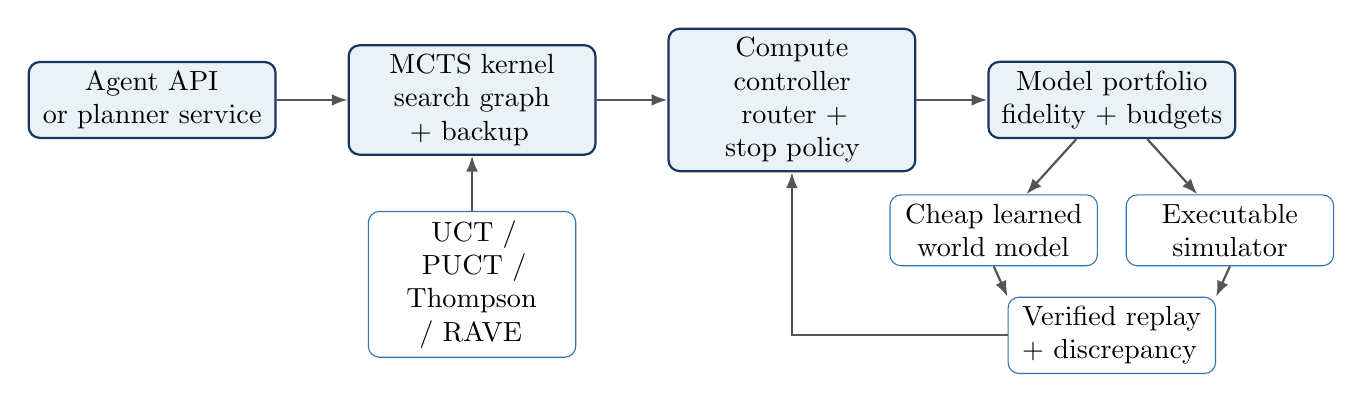
\begin{tikzpicture}[
  node distance=7mm and 9mm,
  box/.style={draw=navy, rounded corners, thick, align=center,
              minimum height=9mm, fill=pale, text width=29mm},
  small/.style={draw=blue, rounded corners, align=center,
                minimum height=8mm, fill=white, text width=24mm},
  arrow/.style={-{Latex[length=2mm]}, thick, draw=graytext}
]
\node[box] (api) {Agent API\\or planner service};
\node[box, right=of api] (kernel) {MCTS kernel\\search graph + backup};
\node[box, right=of kernel] (meta) {Compute controller\\router + stop policy};
\node[box, right=of meta] (portfolio) {Model portfolio\\fidelity + budgets};

\node[small, below=of portfolio, xshift=-15mm] (cheap) {Cheap learned\\world model};
\node[small, below=of portfolio, xshift=15mm] (high) {Executable\\simulator};
\node[small, below=20mm of portfolio] (replay) {Verified replay\\+ discrepancy};
\node[small, below=of kernel] (rules) {UCT / PUCT /\\Thompson / RAVE};

\draw[arrow] (api) -- (kernel);
\draw[arrow] (kernel) -- (meta);
\draw[arrow] (meta) -- (portfolio);
\draw[arrow] (portfolio) -- (cheap);
\draw[arrow] (portfolio) -- (high);
\draw[arrow] (cheap.south) -- (replay.north west);
\draw[arrow] (high.south) -- (replay.north east);
\draw[arrow] (replay.west) -| (meta.south);
\draw[arrow] (rules) -- (kernel);
\end{tikzpicture}
\caption{\method separates MCTS mechanics, algorithmic rules, and meta-level
compute allocation. Cheap and executable evidence are paired in verified
replay.}
\label{fig:architecture}
\end{figure*}

\subsection{Routing and stopping}

A reference score for a feasible compute action is
\begin{equation}
S_\theta(c,h)
=
\widehat{\Delta U}_\theta(c,h)
-\lambda^\top \widehat g_\theta(c,h)
-\kappa \widehat{\rho}_\theta(c,h),
\label{eq:routerscore}
\end{equation}
where \(\widehat{\Delta U}\) predicts decision improvement, \(\widehat g\)
resources, and \(\widehat\rho\) risk. Hard budget masks are applied before
scoring. The router chooses \(\arg\max_c S_\theta(c,h)\) only when the maximum
is positive; otherwise it stops.

Router features include search depth, value gaps, visits, predictive variance,
model disagreement, expected cheap-to-accurate discrepancy, novelty, branch
impact, reversibility, verifier availability, remaining budgets, and service
load. The action may be factorized into branch, model, token budget, horizon,
sample count, and verifier. This permits new portfolio members without
retraining a flat classifier from scratch.

We include simple uncertainty-threshold and fixed-cascade policies as strong
engineering baselines. A learned router earns its complexity only if it
outperforms them under matched budgets.

\subsection{Evidence aggregation and backup}

An evidence aggregator produces a return distribution, not only a scalar.
Candidate implementations are:

\begin{itemize}[leftmargin=1.2em,itemsep=0.15em,topsep=0.25em]
    \item verified-first selection;
    \item Bayesian fusion with model-specific likelihoods;
    \item cheap prediction plus discrepancy posterior;
    \item ensemble disagreement with conservative lower bounds;
    \item direct neural value or mixed value/rollout estimates.
\end{itemize}

The backup interface then chooses mean, distributional, robust, or mixed
propagation. For Crazy Stone compatibility,
\[
V_{\mathrm{robust}}(s)
= Q\!\left(s,\arg\max_a N(s,a)\right),
\]
and
\[
V_{\mathrm{mix}}(s)
=(1-\alpha_s)V_{\mathrm{mean}}(s)
+\alpha_sV_{\mathrm{robust}}(s),
\]
where \(\alpha_s\) can depend on visits and variance. Alternating-agent value
perspective is configured explicitly.

\subsection{Budgeted search procedure}

\begin{figure}[t]
\small
\fcolorbox{navy}{white}{%
\parbox{0.94\columnwidth}{
\textbf{Algorithm 1: Adaptive multi-fidelity MCTS}
\begin{enumerate}[leftmargin=1.35em,itemsep=0.1em,topsep=0.2em]
    \item Synchronize or create the root search graph.
    \item While the resource ledger permits an iteration:
    \begin{enumerate}[leftmargin=1.2em,itemsep=0.05em]
        \item select a path using the injected tree policy;
        \item expand a legal frontier;
        \item build a router context from evidence and budgets;
        \item query feasible compute actions until the router stops;
        \item aggregate evidence into an evaluation distribution;
        \item back up along the explicit iteration path;
        \item append a structured trace and measured usage.
    \end{enumerate}
    \item Select a root task action under the configured decision rule.
\end{enumerate}
}}
\caption{Algorithm-name conditionals are unnecessary. AlphaGo Zero uses direct
neural evaluation plus a no-rollout policy; UCT uses rollouts; adaptive variants
insert model queries before evidence aggregation.}
\label{alg:method}
\end{figure}

The ledger reserves a conservative model quote before a query and commits
measured usage afterward. A model that exceeds its quote triggers a fault policy
rather than silently breaking the search budget.

\subsection{Verified self-improvement}

Whenever executable or real evidence becomes available, the system stores
\[
(h,s,a,m,\hat y_m,\hat \sigma_m,
 c,p(c\mid h),y_H,g,\mathrm{versions}).
\]
This supports four distinct objectives:
\begin{align}
\mathcal{L}_{\mathrm{value}} &=
  \ell(\hat y_m,y_H),\\
\mathcal{L}_{\mathrm{disc}} &=
  \ell(\hat\delta_m,y_H-\hat y_m),\\
\mathcal{L}_{\mathrm{route}} &=
  -\widehat{\mathrm{EVC}}(c,h),\\
\mathcal{L}_{\mathrm{cal}} &=
  \ell_{\mathrm{proper}}(\hat p_m,y_H).
\end{align}
Updates are staged: collect with frozen versions, validate, train candidates,
evaluate offline, run randomized canaries, and promote only after quality,
calibration, cost, and safety gates pass.

Search can also produce visit distributions or verified pairwise rankings for
distillation and preference optimization
\citep{feng2024tsllm,xu2025mctsep}. This can replace the policy-optimization
step of some RLHF pipelines, but not human preference elicitation or reward
validation. Model-only outcomes remain labeled synthetic.

\subsection{Causal logging and evaluation}

Because the router decides what to verify, verified replay is selected data.
We log the probability of every chosen route and allocate bounded randomized
audit traffic. For a deterministic target router \(\pi\), a doubly robust
estimate has the form
\begin{multline}
\widehat V_{\mathrm{DR}}(\pi)
=\frac{1}{n}\sum_{i=1}^n
\left[
\hat r(x_i,\pi(x_i)) \right.\\
\left.
+\frac{\mathbf{1}\{c_i=\pi(x_i)\}}{p_i}
\left(r_i-\hat r(x_i,c_i)\right)
\right].
\end{multline}
Overlap, stable treatment definitions, and sensitivity analyses are required.
Causal claims are limited to interventions the system can define and support.

\section{Software Architecture}

\subsection{MonteCarloGym kernel}

\mcg provides a stable agent interface:
\begin{center}
\small\texttt{action = agent.compute\_action(}\\
\small\texttt{sim\_env, observation)}
\end{center}
The user then calls the normal Gymnasium
\(\texttt{env.step(action)}\) and passes the real transition to
\(\texttt{agent.observe}\). Gymnasium standardizes environment interaction
\citep{towers2024gymnasium}, but generic generative-model protocols keep the
kernel usable outside Gym.

The environment wrapper supports native snapshot/restore, clone state, safe
deep copy, deterministic event reconstruction, or an external model. A
transaction restores internal state, wrapper state, RNG streams, episode
counters, and terminated/truncated flags even after exceptions. Environments
that cannot satisfy this contract fail fast.

The search graph stores statistics on action edges and represents stochastic
outcomes explicitly. Transposition tables use adapter-provided state keys. Tree
reuse re-roots only after a matching real transition and invalidates
incompatible model or state versions.

\subsection{Dependency injection and presets}

The engine depends on protocols for tree policy, expander, evaluator, rollout
policy, backup, model portfolio, compute router, stop policy, reward source,
state codec, and trace sink. Table~\ref{tab:presets} summarizes classical
presets. They share the same engine.

\begin{table*}[t]
\centering
\small
\caption{Classical compatibility presets in the proposed open-source kernel.}
\label{tab:presets}
\begin{tabularx}{\textwidth}{@{}lXXXX@{}}
\toprule
Preset & Selection & Evaluation & Statistics & Backup/sharing \\
\midrule
UCT & UCB1 & random or heuristic rollout & edge \(N,W,Q\) & mean \\
DNG-MCTS / MCBRL & Thompson or root sampling & sampled reward/transition model & Normal-Gamma and Dirichlet & Bayesian update \\
Crazy Stone & soft/Boltzmann & rollout & visits, mean, variance & mean, robust, or mix \\
AlphaGo APV & PUCT & value network plus fast rollout & \(N,W,Q,P\) & mean, neural batching \\
AlphaGo Zero & PUCT & direct policy-value network & \(N,W,Q,P\) & mean, no rollout \\
RAVE / MAST & blended UCT/RAVE & globally biased rollout & direct, AMAF, global move values & direct+AMAF / base backup \\
\bottomrule
\end{tabularx}
\end{table*}

\subsection{Deployment and open-source surfaces}

The dependency-light Python core is distributed through PyPI. A containerized
planner service exposes HTTP/gRPC/MCP interfaces for enterprise and non-Python
agents. Thin TypeScript adapters should expose an explicit
\texttt{plan\_and\_execute} operation rather than assume a late tool hook can
control earlier model selection. Router and discrepancy checkpoints, model
cards, and permitted datasets can be released through model/data hubs.

Production deployments separate search coordinators, batched model gateways,
simulator workers, replay storage, tracing, and asynchronous training. Every
request has a budget envelope and idempotency key. Speculative execution uses a
sandbox or dry run; irreversible or externally visible actions require an
approval boundary.

\section{Experimental Protocol}

The empirical goal is to compare end-to-end planners under equal task
distributions, model portfolios, external-action policies, and budgets. The
task instance, not a tree simulation, is the independent unit.

\subsection{Benchmark ladder}

\begin{table}[t]
\centering
\small
\caption{Planned benchmark ladder.}
\label{tab:benchmarks}
\begin{tabularx}{\columnwidth}{@{}lXXX@{}}
\toprule
Level & Domain & Cheap & Accurate \\
\midrule
L0 & synthetic tree & biased oracle & truth oracle \\
L1 & Gymnasium & learned dynamics & cloned env \\
L2 & tool agents & language world model & code/DB env \\
L3 & web/enterprise & LLM/DOM predictor & browser sandbox \\
\bottomrule
\end{tabularx}
\end{table}

L0 tests identifiability, budgets, and routing invariants. L1 validates the
classical kernel and stochastic state handling. L2 pairs a language world model
such as Qwen-AgentWorld with executable Agent World Model environments
\citep{zuo2026qwenagentworld,wang2026agentworld}. L3 uses BrowserGym and
WorkArena \citep{le2025browsergym,drouin2024workarena}. At least one L1 and one
L2/L3 suite are required for a conference claim.

\subsection{Baselines}

Required comparisons are: direct policy/no search; cheap-only search;
accurate-only search; fixed top-\(k\) cascade; random escalation matched to the
method's call rate; uncertainty threshold; query-level model router; query-level
joint model/token router; \method; and, where computable, an oracle router.
Classical UCT, PUCT, Thompson, robust/mix, RAVE, and MAST controls validate the
implementation.

\subsection{Metrics and primary analysis}

We measure task success, return, regret, constraint satisfaction, tokens,
normalized monetary cost, accurate calls, model calls by tier, environment
steps, compute time, latency quantiles, memory, unsafe attempts, approval
requests, and verifier pass rates. Diagnostics include value error, likelihood,
interval coverage, calibration error, fidelity discrepancy, escalation
precision/recall, stopping regret, and offline-evaluation bias.

The primary result is a success--cost--risk Pareto frontier across at least five
budget levels. We report hypervolume under preregistered reference points,
success at matched cost, cost at matched success, and area under the
budget-performance curve. A single weighted aggregate is secondary.

\subsection{Hypotheses and ablations}

The confirmatory hypothesis is that \method improves Pareto hypervolume over
single-model search and fixed/query-level routing. Secondary hypotheses test
whether discrepancy-aware allocation improves over uncertainty alone, learned
stopping is non-inferior in quality while reducing resources, verified replay
improves held-out calibration, and causally corrected offline estimates better
predict online router rankings.

Ablations remove discrepancy prediction, calibrated uncertainty, executable
verification, token routing, variable depth, stopping, tree reuse, verified
replay, propensity logging, causal correction, risk constraints, and
transpositions. We separately test branch routing without model routing and
model routing without branch routing.

\subsection{Statistics and artifacts}

Task instances and seeds are paired across methods. Synthetic suites use at
least 30 independent seeds; expensive-suite sample sizes follow a
preregistered pilot and power analysis. We use paired, task-stratified bootstrap
intervals, report effect sizes, correct confirmatory comparison families, and
use a non-inferiority margin for stopping claims. Splits are by task family when
possible.

Each run releases its resolved configuration, source revision, environment and
model versions, seeds, structured traces, per-episode JSONL, failures, and
analysis. Provider non-determinism is measured by repeating a subset across
time/load strata. The included L0 scaffold is a software smoke test, not a
reported result.

\section{Discussion}

\subsection{Why this may work}

The method exploits three forms of heterogeneity. First, branch importance is
unequal by construction in tree search. Second, model error is structured:
cheap simulators are often adequate for routine transitions but fail on novel,
ambiguous, or safety-critical states. Third, decision value is thresholded: an
additional observation matters only when it can change the eventual action or
reduce unacceptable risk. EVC gives a common language for these effects.

The architecture also makes enterprise scale plausible. Cheap local models can
provide breadth, expensive services can be reserved for pivotal branches, and
executable sandboxes provide evidence without touching production systems.
Token efficiency becomes an outcome of the compute policy rather than a fixed
global limit.

\subsection{Relationship to RLHF}

Predictive search can serve as policy improvement at inference time or produce
targets for distillation/preference optimization. In this limited sense it can
replace ``the RL step'' of an alignment pipeline. It cannot determine what
humans want, validate a reward model, or guarantee safety. Search may amplify
reward hacking by finding adversarial high-score trajectories. We therefore
retain reward provenance, component scores, uncertainty penalties, independent
verifiers, and human approval for consequential actions.

\subsection{Why causality is optional, not decorative}

Causal correction addresses a concrete problem: the next router is trained and
selected from outcomes acquired by the previous router. Randomized audits and
propensity-based estimators can reduce selection bias. Structured causal world
models may help in domains with stable, intervenable variables. However,
general causal discovery from language traces is weakly identified; imposing a
causal graph can add untestable assumptions and greatly expand scope. The core
requires propensity logging and supports causal estimators, but does not label
every predictive world model causal.

\section{Limitations and Risks}

\paragraph{EVC estimation.}
The value of a computation depends on counterfactual future search, making
supervision sparse and policy-dependent. Simple threshold routers may remain
competitive. Oracle-router experiments are needed to quantify available
headroom.

\paragraph{High fidelity is not ground truth.}
Executable synthetic environments can omit production behavior. Browser
sandboxes can differ from live sites. We must report simulator-real discrepancy
and use real outcomes only where safe and consented.

\paragraph{Distribution shift and feedback loops.}
Verified replay is concentrated near the router's boundary. Without exploration
and correction, the system may become confidently blind elsewhere. Jointly
updating world model and router can destabilize targets.

\paragraph{Safety and security.}
Tree search can generate many tool actions, increasing prompt-injection and
credential exposure. Speculation must be isolated; logs must redact secrets;
side effects must be approval-gated. A sandbox reduces but does not eliminate
risk.

\paragraph{Overhead.}
Maintaining uncertainty, discrepancy, traces, and routing can cost more than it
saves on easy tasks. No-search and fixed-cascade baselines are therefore
essential.

\paragraph{Research breadth.}
The full architecture spans MCTS, routing, world models, causal evaluation, and
agent systems. A first paper should fix one strong simulator pair, one learned
router family, and a limited set of classical controls rather than implement
every advertised extension simultaneously.

\section{Open-Source Plan and Broader Impact}

The codebase will separate a minimal \mcg kernel from optional Gymnasium,
PyTorch, Transformers, browser, and service extras. Source and issues live on
GitHub; Python artifacts on PyPI; service images in an OCI registry; and
permitted checkpoints/data with model cards on a model hub. Versioned research
artifacts can receive archival DOIs.

Positive uses include lower-cost planning, reproducible MCTS research, safer
sandbox-first agents, and better resource accounting. Negative uses include
more capable automation of harmful tasks and reward-model exploitation.
Adapters should default to read-only/dry-run operation, use scoped credentials,
and expose both safety and cost telemetry. Training data and model-generated
traces must be labeled by provenance.

\section{Conclusion}

\method reframes MCTS simulation as a portfolio allocation problem. The planner
must choose not only what an agent should do, but how it should acquire enough
evidence to decide: which branch to inspect, which model to trust, how many
tokens and rollout steps to spend, whether to verify, and when to stop. This
formulation connects classical and neural MCTS, LLM routing, world models,
metareasoning, preference optimization, and targeted causal evaluation while
remaining testable through explicit budgets and Pareto analysis.

The proposed paper succeeds only if experiments show that joint branch-level
control beats simpler routing and cascades on held-out executable tasks. The
open-source architecture and harness are designed to make that claim
reproducible---or falsifiable.

\appendix

\section{API Contracts}

\paragraph{Generative model.}
A model exposes stable identity, fidelity, a conservative pre-call resource
quote, and an evaluation method. Its observation includes value, variance,
measured cost, tokens, latency, risk, optional next state, terminal flags, and
metadata.

\paragraph{Planner.}
The common planner receives a state, model portfolio, hard search budget, and
seed. It returns a task action, predicted value, exact resource usage, and an
auditable structured trace.

\paragraph{Reward source.}
Rules, environment rewards, preference models, humans, and verifiers implement
one scoring protocol. A score carries scalar value, named components,
verification status, source, and version.

\paragraph{Replay.}
A verified record pairs cheap predictions with executable or real outcomes and
includes router propensity. Synthetic, executable, and real provenance are
never collapsed.

\section{Implementation Invariants}

\begin{enumerate}[leftmargin=1.4em,itemsep=0.15em]
    \item Snapshot/restore reproduces environment and RNG state.
    \item Planning cannot mutate the live environment.
    \item Edge visits equal completed backups.
    \item Resource limits are never exceeded, including failures.
    \item Termination and truncation remain distinct.
    \item Robust max selects the most-visited child.
    \item Imaginary Bayesian transitions do not update the real root belief.
    \item RAVE direct and AMAF updates are not double counted.
    \item Accurate evidence augments rather than silently overwrites provenance.
    \item Every learned route used for causal evaluation has a logged propensity.
\end{enumerate}

\section{Submission Readiness Checklist}

Before replacing this draft's proposal language with empirical claims, require:
one Gymnasium and one executable agent suite; all matched-budget baselines; at
least five budget levels; held-out task-family evaluation; router and
discrepancy ablations; calibration and safety reporting; paired uncertainty
intervals; model/token/simulator cost accounting; and released configurations,
code, and representative structured traces.

\balance
\bibliographystyle{plainnat}
\bibliography{references}

\end{document}
